\documentclass{article}
\usepackage{hyperref}
\usepackage{amsmath, amssymb}
\setlength{\parindent}{3ex}
%Includes "References" in the table of contents
\usepackage[nottoc]{tocbibind}
\usepackage[utf8]{inputenc}
%\usepackage[style=authoryear-ibid,backend=biber]{biblatex}
\usepackage[style=numeric,backend=biber]{biblatex}
\addbibresource{self-ref-2026.bib}

\usepackage[italicdiff]{physics}
\usepackage{tikz}
\usetikzlibrary{arrows,automata, positioning}
\usepackage{float}
\usepackage[english]{babel}
\usepackage[strict]{csquotes}% Recommended
\usepackage{braket} %Dirac notation
\usepackage[hmarginratio=1:1,top=32mm,columnsep=20pt]{geometry} % Document margins
\setlength{\parskip}{0.5em}
\usepackage{multicol} % Used for the two-column layout of the document
\usepackage{booktabs}
%\usepackage{quotchap}
\title{It from Bit via G\"odel - Part 1}
\author{ John Small
}
\date{\today}

\begin{document}

\maketitle

\medskip

\noindent\rule{\textwidth}{0.4pt}
\begin{abstract}
  Quantum states have the curious property that are exactly what's required to represent the classically impossible states which occur in proofs of non-computability and undecidability, which in turn rely on in self-reference. This is a pretty big clue to understand what quantum states actually are. We follow that clue in an attempt to uncover an insight into John Wheeler's question "How come the quantum?". If a new insight is to be worth anything then it must enable us to answer hard questions and calculate numbers we can compare with experiment. And it does. We find a rationale for the 3 dimensions of space, for the symmetry groups of the Standard Model, a valuable duality between multiparticle entanglement and the Standard Model via Hopf fibration which enables us to  understand why the strong force ignores parity and do a preliminary calculation of free parameters. The duality also enables us to create some simple quantum circuits for particle interactions. There are many gaps in the project and we list a number of open problems.
\end{abstract}
\noindent\rule{\textwidth}{0.4pt}

\section{Introduction}
This paper contains few new theorems. Where there is novelty it is only in finding connections between already established theorems and then filling the gaps. To find such connections we use a simple principle, underlying self-refence, or acausality forced into an overlying non-self-referent causal framework. Surprisingly this enables us to spot connections which others have guessed at and yet not persued.

\subsection{Principal Results}
\label{sec:results}

The framework yields three classes of result: structural derivations of Standard Model architecture (gauge group, particle content, spacetime dimensionality), quantitative predictions for masses and couplings, and falsifiable non-observation predictions. We summarise each in turn.

\subsection{Structural results}

The following structural features of the Standard Model are derived, not assumed:

\begin{enumerate}
  \item \textbf{Gauge group.} The Standard Model gauge group $G_{\mathrm{SM}} = SU(3) \times SU(2) \times U(1)/\mathbb{Z}_6$ is the equivariance group of the octonionic Hopf fibration $S^7 \to S^{15} \to S^8$ after selection of the preferred complex direction $\mathbb{C} \subset \mathbb{O}$ forced by the Moufang loop closure (Section~\ref{sec:gauge}).

  \item \textbf{Particle content.} The complete Standard Model particle spectrum is in bijection with the entanglement primitives of three Cayley--Dickson qubits (Table~\ref{tab:dictionary}), with exhaustiveness guaranteed by three independent termination theorems: Hurwitz (no division algebras beyond~$\mathbb{O}$), Adams (no Hopf fibrations beyond the octonionic case), and Coecke--Kissinger (compositional completeness of GHZ and W classes).

  \item \textbf{Spacetime dimensionality.} The requirement that state reduction on the Bloch sphere be consistent with Lorentz boosts demands $\mathrm{Spin}(1,d) \cong SL(2,\mathbb{A})$ for a normed division algebra~$\mathbb{A}$. The computability split selects $\mathbb{A} = \mathbb{C}$, giving $SL(2,\mathbb{C}) = \mathrm{Spin}(1,3)$ and thus $d = 3$ spatial dimensions. The six internal dimensions of $SU(3) \times SU(2) \times U(1)$ account for the reduction from $d = 9$ (the octonionic case) to $d = 3$, reproducing the Kaluza--Klein dimensional decomposition $9+1 = (3+1) + 2 + 4$ with a structural explanation.

  \item \textbf{Three generations.} The triality automorphism of $\mathrm{Spin}(8)$, which permutes the three eight-dimensional representations of the octonions, produces exactly three generations of fermions.

  \item \textbf{Chirality.} The non-associativity of $\mathbb{O}$ distinguishes left and right multiplication, breaking parity at the algebraic level.

  \item \textbf{Born rule.} The observer's self-referential ignorance of their own computational state generates a global $U(1)$ phase freedom. The minimum-degree polynomial invariant under this symmetry is $|\psi|^2$, yielding the Born rule without additional postulates (Section~\ref{sec:born}).

  \item \textbf{Entanglement monogamy.} The Coffman--Kundu--Wootters inequality follows geometrically from the compactness of the $S^4$ base of the quaternionic Hopf fibration: a ball has a unique centre, and one cannot overshoot it (Section~\ref{sec:monogamy}).
\end{enumerate}

\begin{table}[t]
  \centering
  \caption{Entanglement class $\leftrightarrow$ particle type dictionary. Exhaustiveness is guaranteed by the termination of Hopf fibrations at the octonionic case (Adams' theorem) and the compositional completeness of GHZ and W classes (Coecke--Kissinger theorem).}
  \label{tab:dictionary}
  \begin{tabular}{lll}
    \toprule
    Entanglement class & Particle type & Physical property \\
    \midrule
    Product state & Higgs field & Sets vacuum entanglement convention \\
    Bell (2-qubit) & Gauge bosons & Mediate bipartite correlations \\
    GHZ (3-qubit) & Quarks & All-or-nothing $\to$ confinement \\
    W (3-qubit) & Leptons & Distributed pairwise $\to$ free particles \\
    \bottomrule
  \end{tabular}
\end{table}

\subsection{Quantitative predictions: fermion masses}

The mass of each charged fermion is given by the generalised Koide formula
\begin{equation}
  \label{eq:koide}
  \sqrt{m_k} \;=\; M\!\left(1 + \alpha\cos\!\left(\delta + \frac{2\pi k}{3}\right)\right), \qquad k = 0, 1, 2\,,
\end{equation}
where $k$ labels the three generations within each charge sector. The two dimensionless parameters $\alpha$ and $\delta$ are determined by quantum numbers as follows.

\paragraph{Koide angle.} The misalignment between the triality-symmetric direction on $\mathbb{O}P^1$ and the preferred complex direction gives
\begin{equation}
  \label{eq:delta}
  \delta_{\mathrm{sector}} \;=\; \frac{\delta_0}{n}\,, \qquad \delta_0 = \frac{\dim_{\mathbb{R}}(\mathbb{C})}{\dim_{\mathbb{R}}(\mathbb{O}P^1)} = \frac{2}{9}\,,
\end{equation}
where $n$ counts the number of active internal fibre directions:
\begin{equation}
  n \;=\; 1 + \bigl(T_3 + \tfrac{1}{2}\bigr) + \mathbf{1}_{\mathrm{colour\,triplet}}\,.
\end{equation}

\paragraph{Amplitude parameter.} The ratio of rotation to identity components in the SU(2) holonomy of the self-referential loop gives
\begin{equation}
  \label{eq:alpha}
  \alpha^2 \;=\; 2 + 2\,|Q|^{3/2}\,\mathbf{1}_{\mathrm{colour\,triplet}}\,,
\end{equation}
where $|Q|$ is the magnitude of the electric charge. For charged leptons, $\alpha = \sqrt{2}$ corresponds to a quarter-turn ($\pi/2$) holonomy.

\paragraph{Dimensional parameter.} Each charge sector has one free dimensional parameter $M$, fitted to the heaviest observed mass ($m_\tau$, $m_b$, $m_t$). All mass \emph{ratios} within a sector are therefore predictions with zero free parameters.

Table~\ref{tab:inputs} summarises the sector-specific inputs. Table~\ref{tab:masses} presents the resulting mass predictions, and Table~\ref{tab:ratios} presents inter-generation mass ratios.

\begin{table}[t]
  \centering
  \caption{Sector-specific parameters. All dimensionless quantities ($\alpha$, $\delta$) are determined by quantum numbers; only the dimensional scale $M$ is fitted (to the heaviest mass in each sector).}
  \label{tab:inputs}
  \begin{tabular}{lccccccc}
    \toprule
    Sector & $|Q|$ & $T_3$ & Colour & $n$ & $\delta$ & $\alpha^2$ & $M$ fitted to \\
    \midrule
    Charged leptons & 1 & $-\tfrac{1}{2}$ & singlet & 1 & $2/9$ & 2 & $m_\tau$ \\
    Down-type quarks & $\tfrac{1}{3}$ & $-\tfrac{1}{2}$ & triplet & 2 & $1/9$ & $2 + 2/3\sqrt{3}$ & $m_b$ \\
    Up-type quarks & $\tfrac{2}{3}$ & $+\tfrac{1}{2}$ & triplet & 3 & $2/27$ & $2 + 2\sqrt{2/3\sqrt{3}}$ & $m_t$ \\
    \bottomrule
  \end{tabular}
\end{table}

\begin{table}[t]
  \centering
  \caption{Charged fermion mass predictions. Eight of nine masses are reproduced to better than 1.1\% from the single dimensionless constant $\delta_0 = 2/9$ and the quantum numbers of each particle. The up quark discrepancy has an identified mechanism (see text). Measured values from the Particle Data Group~\cite{PDG2024}; light quark masses are $\overline{\mathrm{MS}}$ at $\mu = 2\;\mathrm{GeV}$.}
  \label{tab:masses}
  \begin{tabular}{lrrr}
    \toprule
    Particle & Predicted (MeV) & Measured (MeV) & Deviation \\
    \midrule
    $e$ & 0.5110 & 0.5110 & $-0.01\%$ \\
    $\mu$ & 105.652 & 105.658 & $-0.01\%$ \\
    $\tau$ & 1776.86 & 1776.86 & fitted \\[4pt]
    $d$ & 4.62 & 4.67 & $-1.0\%$ \\
    $s$ & 94.4 & 93.4 & $+1.1\%$ \\
    $b$ & 4180 & 4180 & fitted \\[4pt]
    $u$ & 2.78 & 2.16 & $+28.5\%\;^{(*)}$ \\
    $c$ & 1271.4 & 1270 & $+0.1\%$ \\
    $t$ & 172\,500 & 172\,500 & fitted \\
    \bottomrule
    \multicolumn{4}{l}{\footnotesize $^{(*)}$ See Section~\ref{sec:upquark} for the identified W-class interference mechanism.}
  \end{tabular}
\end{table}

\begin{table}[t]
  \centering
  \caption{Inter-generation mass ratios (zero free parameters). All ratios except $m_c/m_u$ are predicted to better than 2\%. The $m_c/m_u$ discrepancy shares the same origin as the up quark mass anomaly.}
  \label{tab:ratios}
  \begin{tabular}{lrrr}
    \toprule
    Ratio & Predicted & Measured & Deviation \\
    \midrule
    $m_\mu / m_e$ & 206.8 & 206.8 & $0.006\%$ \\
    $m_\tau / m_e$ & 3477.5 & 3477.2 & $0.008\%$ \\[4pt]
    $m_s / m_d$ & 20.4 & 20.0 & $2\%$ \\
    $m_b / m_d$ & 903.9 & 895.1 & $1\%$ \\[4pt]
    $m_t / m_c$ & 135.68 & 135.83 & $0.1\%$ \\
    $m_c / m_u$ & 458 & 588 & $22\%\;^{(*)}$ \\
    \bottomrule
  \end{tabular}
\end{table}

\paragraph{The up quark anomaly.} The up quark is the only fermion where the $T_3 = +\tfrac{1}{2}$ member is lighter than the $T_3 = -\tfrac{1}{2}$ member ($m_u < m_d$). In generations~2 and~3, the pattern reverses: $m_c \gg m_s$ and $m_t \gg m_b$. This generation-1 flip emerges from the competition between two effects: the amplitude parameter~$\alpha$ (larger for up-type quarks due to $|Q| = 2/3$) stretches the mass scale upward, while the dilution of the Koide angle (smaller $\delta$ for up-type quarks, $n = 3$ vs $n = 2$) suppresses the lightest generation more strongly. At generation~1, the $\delta$~suppression dominates; at generations~2 and~3, the $\alpha$~enhancement dominates. However, the quantitative prediction for $m_u$ overshoots by 28.5\%, indicating that a correction from the interference between GHZ (tripartite) and W (pairwise) entanglement contributions --- which are comparable in magnitude only at generation~1 --- must be included. This calculation is identified as an open problem (Section~\ref{sec:open}).

\subsection{Quantitative predictions: bosonic sector}

The framework yields the following zero-parameter predictions for bosonic quantities:

\begin{table}[h]
  \centering
  \caption{Bosonic sector predictions. All values are derived from the Hopf fibration geometry with no free parameters. The Weinberg angle and strong coupling are tree-level predictions; measured values include radiative corrections via standard renormalisation group evolution with Standard Model particle content.}
  \label{tab:bosons}
  \begin{tabular}{llll}
    \toprule
    Quantity & Predicted & Measured & Deviation \\
    \midrule
    $\sin^2\!\theta_W$ & $1/4$ (tree level) & 0.2312 (at $M_Z$) & consistent after RGE \\
    $m_H$ & $v/2 = 123.1\;\mathrm{GeV}$ & $125.25\;\mathrm{GeV}$ & $\sim 2\%$ \\
    $y_t$ (top Yukawa) & 1 & 0.991 & $\sim 1\%$ \\
    $\alpha_s(M_Z)$ & $\approx 0.1185$ & 0.1179 & $\sim 0.5\%$ \\
    $\theta_{\mathrm{QCD}}$ & 0 (topological) & $< 10^{-10}$ & consistent \\
    \bottomrule
  \end{tabular}
\end{table}

The Weinberg angle prediction $\sin^2\!\theta_W = 1/4$ arises from the equal-weight projection on the $S^4$ base of the quaternionic Hopf fibration. This is a tree-level (UV) value; running to $M_Z$ via the standard one-loop renormalisation group equations with the known Standard Model particle content yields $\sin^2\!\theta_W(M_Z) \approx 0.231$, in agreement with the measured value.

The strong CP angle $\theta_{\mathrm{QCD}} = 0$ is topologically forced: the GHZ entanglement class characterising quarks has maximal three-tangle ($\tau_3 = 1$) and zero pairwise concurrence, precluding the oriented linking structure that would generate a non-trivial vacuum angle.

\subsection{Non-observation predictions}

In addition to the quantitative predictions above, the framework makes several structural predictions that take the form of strict non-observations:

\begin{enumerate}
  \item \textbf{No supersymmetric partners.} The division algebra tower terminates at $\mathbb{O}$; no algebraic structure exists to support a boson$\leftrightarrow$fermion symmetry. Confirmed by LHC Run~1 and Run~2 null results.

  \item \textbf{No proton decay.} The gauge group $G_{\mathrm{SM}}$ arises from parallelisable spheres, which do not produce $SU(5)$ or any other simple group containing $G_{\mathrm{SM}}$. Baryon number violation via leptoquark exchange is therefore structurally absent. Consistent with Super-Kamiokande bounds ($\tau_p > 10^{34}$~years).

  \item \textbf{All FCNC top quark decays via neutral bosons are exactly zero at all orders.} Generation labels correspond to triality sectors (associator bracketings); neutral bosons ($Z$, $\gamma$, gluon, Higgs) have no mechanism to change braceting. This is a structural prohibition, stronger than the SM's GIM cancellation. All ATLAS Run~2 searches are consistent with null results. The HL-LHC programme will probe BSM-enhanced rates of $10^{-5}$--$10^{-4}$; the framework predicts these searches will remain null.

  \item \textbf{Neutrino mass sum $\Sigma m_\nu = 2.6\;\mathrm{meV}$, normal ordering.} Testable by DESI, Euclid, and CMB-S4 within the next decade. An inverted mass ordering would falsify the framework.
\end{enumerate}

\subsection{Parameter counting}

The Standard Model has 19 free parameters (or 26 including neutrino masses and mixing). The present framework replaces all dimensionless parameters with derived quantities:

\begin{itemize}
  \item The gauge group is derived (eliminating three coupling constant choices).
  \item The Weinberg angle, Higgs mass, and strong CP angle are predicted.
  \item All charged fermion mass \emph{ratios} follow from $\delta_0 = 2/9$ and quantum numbers.
  \item The CKM and PMNS mixing matrices are structurally constrained (CKM small because GHZ contextual extraction is basis-dependent; PMNS large because W transfer is democratic).
\end{itemize}

The framework retains \textbf{exactly one free dimensional parameter}: the overall mass scale, identified with the Higgs vacuum expectation value $v$. This single free parameter is a structural necessity --- the observer cannot determine the absolute scale of their own computational network by the same self-referential logic that generates quantum mechanics. The theory therefore has one free dimensional parameter and zero free dimensionless parameters.

\section{What is a quantum state?}
\subsection{The problem}
The interminable question that has vexxed minds over the last hundred years lies right at the foundation of our understanding of physical law. Pehaps the clearest and most succinct comment on the subject is from E.T. Jaynes \cite{Jaynes_89_a}
\begin{quotation}
  Because this position seems to arouse fierce controversy, let me stress our motivation: if quan-
  tum theory were not successful pragmatically, we would have no interest in its interpretation. It is
  precisely because of the enormous success of the QM mathematical formalism that it becomes crucially important to learn what that mathematics means. To find a rational physical interpretation
  of the QM formalism ought to be considered the top priority research problem of theoretical physics;
  until this is accomplished, all other theoretical results can only be provisional and temporary.
\end{quotation}
In the same article he follewed it up with ;-
\begin{quotation}
  But our present QM formalism is not purely epistemological; it is a peculiar mixture describing
  in part realities of Nature, in part incomplete human information about Nature all scrambled up
  by Heisenberg and Bohr into an omelette that nobody has seen how to unscramble. Yet we think
  that the unscrambling is a prerequisite for any further advance in basic physical theory. For, if we
  cannot separate the subjective and objective aspects of the formalism, we cannot know what we
  are talking about; it is just that simple.
\end{quotation}

So the first task is to unscramble the quantum omelette so we know what we are talking about and we have some pretty good clues to work with. The first and most obvious is that through superposition a quantum state can represent the classically inadmissible states which occur in self-referential systems, such as a computer halting and not halting at the same time \cite{Turing} or a statment being true and false at the same time ref(godel). In addition if we look intensly at the \textquote(quantum omlette), the density matrix,  we notice that we can move smoothly between an entirely mixed state which is classical, and therefore epistemological probability, and a quantum pure state where indeterminacy is understood to be an innate feature of nature and therefore ontological. Yet the different points of view describe the same physical situation and the shift between them is entirely dependent on an observer's change in their state of knowledge. Taken together this suggests we should be thinkinng in terms of a self-referential state of knowledge.

But to suggest that our inability to predict the momement a radioactive nucleus decays is due to our own ignorance seems crazy. And yet, the quantum Zeno effect (refs) where some quantum state is prevented from decay into another state by continually checking to see if it has decayed or not, which is continually updating an observer's state of knowledge, hints that just maybe the observer's state of knowledge is not entirely disconnected from a seemingly ontological state of nature.

In addition we note that the $U(1) \times SU(2) \times SU(3)$ symmetry group of the standard model is in some peculiar way linked to the division algebras and hence to parallelisable spheres, yet self-refence requires information flowing round in circles, which requires the parallelisable property. Could there be a connection? The idea is clearly crazy, and yet so tantalising as to be worthy of deeper investigate.

\subsection{Underground connections}
The plain fact that $\ket{TRUE} + \ket{FALSE}$ is a perfectly valid quantum state which can represent a fixed point of self-referential paradoxes such as the Liar Paradox or more formally, the classically invalid states which occur in self-referential systems in Godel's Theorems or Turing's proof of the insoluability of the halting problem has not gone unnoticed. There is the famous story of John Archibald Wheeler on a TWA flight returning to Princeton from Europe suddenly thinking \cite{Wheeler1974}
\begin{quotation}
  Add "paricipant" to "undecidable propositions" to arrive at physics
\end{quotation}
When he got back to Princeton he immediately went to G\"odel's office to explain the idea, but G\"odel was so annoyed he threw him out. Nevertheless, Wheeler developed his idea into the phrase "It from bit,and bit from it". Over the years many people have approached the notion of self-reference being in some ways fundamental. This is not the place for a full literature review, Karl Svovil's book \textquote{Physical Acausality} does a fairly complete job. More recent, and highly relevant is Szangolies \cite{szangolies_2020}. Then there's my own earlier attempt at grappling with these issues in \cite{small_2006}.

Self-reference is important in quantum interpretations because all interpretations and toy models must at some point find a way to accomodate $\ket{TRUE} + \ket{FALSE}$. Therefore the idea is the secret underground connection that unites seemingly quite different views of quantum mechanics. Usually the authors of interpretation X introduce self-reference without realising it or acknowledging it. It pops up in different disguies. In the Many Worlds Interpretation it takes the form of the Axoim of Choice, which implicity draws in an imagined supertask to complete an infinite number of choices in a finite interval of time (refs), in the retro-causal interpretation it takes the form of imagined closed timelike loops, in the Bohmian interpretation it takes the form of non-locality. Penrose is one of the few authors who deliberatly introduce non-computability into their framework. All interpretations of quantum mechanics are trying to impose a causal, computable narrative onto an underlying acausal, non-computable reality, and there's alway a bit that doesn't fit. Frauchiger and Renner~\cite{Frauchiger_2018} proved that all interpretations of quantum mechanics are inconsistent in some way. Which is obvious because you can't fit an underlying acausal, non-computable reality into a causal, computable framework. Just like nailing down a carpet that's too big for a room, there will always be bump left over, all interpretations of Quantum Mechanics are an attempt to nail down an essentially non-computable carpet to fit inside a comptutable room, it won't fit, there's alway a bump left over.
\begin{figure}[H]
  \centering
  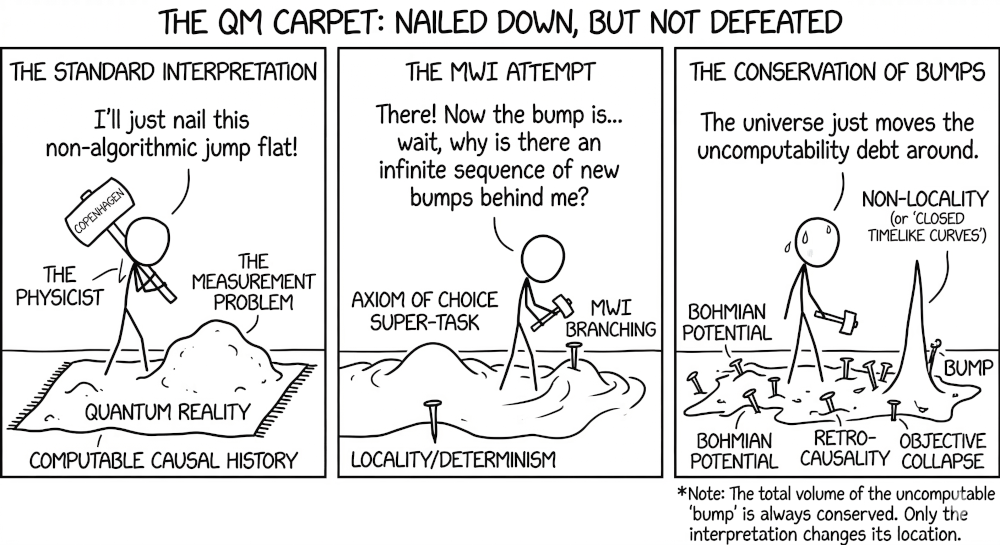
\includegraphics[width=0.85\linewidth]{Gemini_Generated_Image_scaled.png}
  \caption{There's always an inconsistency somewhere}
  \label{fig:myimage}
\end{figure}
The fact that Quantum Mechanics cannot be nailed down to fit our notions of computability is not a bug,  it's feature we can make use of. Recognising that non-computabilty in its various disguises has to be smuggled in to any interpretation or toy model of quantum theory relieves us of the burden of trying to find \textquote{The One True Interpretation}, there isn't one. Instead we can focus on the more modest goal of finding a useful theory we can do calculations with that might open up some hard problems.

It is important to go through each of the different intepretations and toy models to find the point where they smuggle in self-reference, non-computability or acausality. But it's a tangent to the main thread of this article which is to use that idea to do some calculations to get numbers that can be compared with experiment. So I've made a few suggestions for the more popular interpretations in appendix \ref{appendix:interpretatons}, for anyone to work on.

Each intepretation of quantum mechanics has its value in understanding some particular facet of nature, but we shouldn't restrict our affections to just one interpretation. In the same way we freely switch between different coordinate systems, cartesian, spherical or cylindrical according to the task at hand we are free to switch between different interpretations according to the task at hand.We can even switch between entirely different philosophical narrative coordinate systems as we please. We can be epistemologists in the morning, ontologists in the afternoon, and followers of Many Worlds in the evening after few beers. Each has its place and each reveals something useful.

We should take the advice of the great philosopher Groucho Marx~\cite{DuckSoup1933}
\begin{quotation}
  Those are my principles, and if you don't like them... well, I have others.
\end{quotation}
And the same sentiment, but with greater erudition from Edward Gibbon~\cite{Gibbon1776}
\begin{quotation}
  The various modes of worship which prevailed in the Roman world were all considered by the people as equally true; by the philosopher as equally false; and by the magistrate as equally useful.
\end{quotation}
We will take the magistrate's view. Is it useful? As this paper progresses we will freely switch between different interpretations as is useful for the problem at hand.

\subsection{Karl Popper nails it}
Returning to the task set by Jaynes, unscrambling the quantum omlette, and here we have a great thought experiment from 1950 by Karl Popper to guide us, \cite{Popper1950b, Popper1950a}. It's worth looking closely at what he proposed because it contains all the essential elements required to understand why we use complex probability amplitudes in the density matrix, and why they have an epistemological origin. In a terrible irony, having laid the foundations to develop a rationale for an epistemological origin of quantum probablity amplitudes, Popper then spent the rest of his life arguing against any epistemological view of the matter (refs). In his 1950 paper he didn't set out to derive quantum mechanics, the purpose was to show that non-determinism exists even in classical mechanics, if we introduce self reference. The paper was written before electronic computers were a commonplace fact of life and he describes a mechanical computer, like a Babbage-Lovelace analytical engine, which is endowed with the ability to peform all kinds of calculations. We feed into it all the information it needs to calculate the future trajectory of some object, and then get it to calculate the result of an interaction between the object and itself. It can't do it. He writes
\begin{quotation}
  It is usual asserted (I think correctly) that the physical processes involved in observation lead to difficulties only in quantum physics and that they disappear if it is assumed that Plank's quantum of action equals zero - in other words classical physics. Nevertheless I contend that, if in a similar way, we analyse besides the physical processes involved in observation certain other physical processes which are involved in every prediction, then we find a somewhat similar result which, however, is valid for classical physics also. The processes which our analysis must take into account besides observation are the physical processes involved in the calculation and formulation of the predictions. If this is done then we find that all scientific predictions are in an important sense deficient, including the most complete set of predictions possible to formulate even from classical physics; and we find that this deficiency becomes significant whenever we wish to predict the behaviour of physical systems (classical or otherwise) of a certain kind, viz, predicting machines.

  Our procedure will be to consider some of the properties, and especially the limitations, of what we shall call the \textquote{predictor}, i.e. a classical mechanical calculating and predicting machine which is so constructed as to produce permanent records of some kind (such as a tape with holes punched in it) capable of being interpreted as predictions of the positions, velocities and masses of physical particles. It will be shown that such a machine can never fully predict every one of its own future states and consequently not those of what we shall call its (closer) \textquote{environment}, i.e. the part of the world with which it (strongly) interacts. Such a machine, moreover, can never fully predict, or be predicted by, any sufficiently similar machine with which it interacts. ...
  \par
  \hfill \autocite[p.~118]{Popper1950a}
\end{quotation}
\par
He describes a classical mechanically operating \textquote{predictor} $C$ which is set the task of predicting the result of interaction with its closest environment, we might say the result of a future interaction with one element of its environment $E$ about which it has been programmed with complete information. Here it is appropriate to use the epistemological view of probability as expused by E. T. Jaynes because because the predictor is attempting to calculate the outcome of a future interaction between itself $C$ and an external entity $E$ and that predictoin requires information encoded in the physical state of the predictor. This also corresponds with Rovelli's understanding that a quantum measurement never reveals the state of a thing itself, only the relationship between a thing and and an observer \autocite{Rovelli1996a}. Quantum mechanics is about relationships hence it's called the \textquote{relational view of quantum mechanics}  We might consider the predictor $C$ to be a very visibly classical mechanism, such as a Babbage Analytical Engine \autocite{babbage}. Popper then writes;-
\begin{quotation}
  Now if it is impossible for $C$ completely to predict its state (i.e. that of its tape) for \emph{any} moment of its future, we may have to conclude that it will also be impossible for it to predict completely the state of its closest environment.
  \par
  \hfill \autocite[p.~178]{Popper1950a}
\end{quotation}
\par
Replacing \textquote{its closest environment} with $E$ for \textquote{External Entity} we can see that because $C$ cannot predict its own future state then it cannot predict the outcome of an interaction with $E$, i.e. a measurement of $E$. But since the outcome of a measurement is co-determined by $E$ and $C$ together then $C$ can just as well calculate a probability for the outcome of the measurement by assuming that it does have perfect knowledge of its own state at the moment of interaction and the indeterminate result  of a future measurement is in consequence of the nature of $E$ alone. Something Jaynes calls \textquote{the mind projection fallacy} \cite{Jaynes1989}
\begin{quotation}
  It is very difficult to get this point across to those who think that in doing probability calculations
  their equations are describing the real world. But that is claiming something that one could never
  know to be true; we call it the Mind Projection Fallacy. The analogy is to a movie projector,
  whereby things that exist only as marks on a tiny strip of film appear to be real objects moving
  across a large screen. Similarly, we are all under an ego driven temptation to project our private
  thoughts out onto the real world, by supposing that the creations of one's own imagination are real
  properties of Nature, or that one's own ignorance signals some kind of indecision on the part of
  Nature.
\end{quotation}

Popper then goes on to introduce another predictor $C^+$, having the same mechansiums as $C$. This new predictors, $C^+$ is provided with the initial state of $E$ and $C$ and proceeds to calculate the future motions of all the components. From the point of view of $C^+$ the interaction between $E$ and $C$ is completely deterministic, there is no sudden jump in state when $C$ interacts with $E$. $C^+$ succeeds in calculating the outcome of the interaction between $E$ and $C$ with perfect accuracy, and calculates that after the interaction $C$ and $E$ are correlated. But it would find that it can't calculate an outcome of its own future interaction with the combined state of $C$ and $E$. This is the famous example of \enquote{Wigner's friend} \autocite{Wigner1961} implemented in a series of classical Babbage Analytical engines. Since both $C$ and $C^+$ are Universal Turing Machines and therefore have equivalent computing power why is $C^+$ able to calculate something which $C$ can't?
Popper writes;-
\begin{quotation}
  ... But while the fullest information available to $C$ still gives rise to questions about $C$ which $C$ cannot answer, it appears that $C^+$ can posses, in principle, such information about $C$ (and especially $C$'s limitations) as to be able to answer every physical question about $C$
  \par
  Since all this appears to hold for a $C^+$ which is not constructively inferior to $C$, it clearly suggests that \emph{$C$'s inferior knowledge is due to the logical impossibility of imparting it information about itself without, by this very act, making this information obsolete}
  \par
  \hfill \autocite[p.~188]{Popper1950a}
\end{quotation}
I've emphasised \textquote{{\emph{$C$'s inferior knowledge is due to the logical impossibility of imparting it information about itself without by this very act, making this information obsolete}}} because this is Popper's critical insight. Now, at this point it would be nice if someone had proved that self-reference implies complex probabilities, then I could just refer to that work and move on. But although the literature on self-reference and non-computablity is quite voluminous (refs), and the literature on negative, extended or as it is quaintly called "quasi-probability" is also voluminous (refs). There's very little overlap between the fields and certainly no one text I can point to that proves the connection. As this connection is crucial to the rest of this article, it has to support an enormous weight then it's essential to get that right. So we have to assemble the pieces of the jigsaw to see which pieces are missing and then fill in the gaps. The pieces form an imperfect fit and there are quite large gaps.

\subsection{Self-reference and complex probability amplitudes}
The first thing to notice is the scale at which self-reference becomes relevant for $C$ to know the disposition of its own components. If we imagine that $C$ is a giant steam powered Babbage-Lovelace analytical engine then it only becomes important for $C$ to have self-knowledge of its own components when the thing that $C$ is interacting with acts at the same scale as the smallest cog or lever. The time evolution of $C$ is in some state space, and the smallest quantity that would change its path through that state space must therefore have the dimension of action.

When $C$ interacts with a large heavy cannonball the disposition of the tinnest cog is irrelevant and so $C$'s self-knowledge of its own components is not required. But for a very small ball bearing with just enough energy and momentum to flip the tiniest lever or disturb the tiniest cog and for the lever and tiniest cog to have a back reaction on the very small ball bearing then $C$'s self knoweldge of its own components is required. Therefore there will be a scale at which it becomes impossible for $C$ to predict the outcome of its interaction with its closest environment and that scale will have the dimension of action.

From that we can deduce that when we try to nail down the carpet of non-computability in the room of computability the nail will enforce a barrier to knowing the most minute details of any action. So we should expect to find articles which frame self-reference in terms of a fundamental limit to knowledge, an \textquote{Epistemic Horizon} \cite{szangolies_j_2018, szangolies_2020} or ref(spekkens toy model)

The second thing to note that $C$'s act of knowing its own state simultaneously erases that state implicitly assumes performing an infinite number of actions in a finite amount of time, which is the definition of a supertask, and the definition of a supertask requires the completion of $\mathbb{R}$, and hence continuity.

The third thing to note is that \textquote{without by this very act, making this information obsolete} we assume we can go back and erase something that has happened. So we expect to find reversibility and negative probabilty.

List articles on negative probability in general
List articles on negative probability and QM.
List articles on self-reference in QM
List articles that indirectly join together self-reference and negative probability via contextuality
Point out that these are phenomenological, they described phenomena without grounding it in a principle.
So we're circling close, but there seems to be an insight missing.
Re-examine Burgin and identify that negative probabilty has to be private knowledge because it cannot form records. Entropy etc. Introduce the FANOUT as the distinction between public and private.
Now we're getting close, $C$ inability to predict is due to an in principle lack of knowledge of its own state and because it cannot form a shareable record it has to be a negative probabilty. Private state of knowledge about its own state (find Qbist quote)
Point out that despite objections we are forced to use Shannon Information theory because the probabilty is due to an in principle deficity of information. Therefore we have to analytically continue to the complex plane. So we get neg prob and prob > 1.
Bring that back to Spencer-Brown, Kauffman and Russel Paradox and the resolution of Russel's Paradox and hence all Lawver/Yanofsky paradoxes.
Note that it means all paradoxes require complex information. Which means that we can ask about distance between computable and non-computable states.
Introduce paralellisable spheres. complex states Bloch sphere, S1 fibre is the unobservable global phase
But first show derivation of postulates of quantum mechanics.



Then move on to explore notions of computable distance. Set up computational model and define non-computable distance as requiring 'as if' CTCs. Point out that this means parallelisables spheres, but only up to 3d because of non-associativity of octonions.

Point out that toy model, can help see features of GR.
1) relationalist
2) depends on the density of compution, more space where more computation
3) Bell state before measurement is outside the network
4) Measurement creates spacetime for the measurement to happen in
5) Even though S7 can't be used for a metric space, it hasn't gone away and the information exchanged between events must be constrained by algebra of S7

Switch to GR
1) Electon in a bottle.
2) measurement creates ST in which to happen. (hilbert hotel) Tips light cone, changes causal structure, acceleration, creates new spacetime.
3) Dresssing a non-computable event as if it's the result of a computable process
4) Light cone tipping and Unruh effect
5) 7 lefts = 1 right from octonions. measurement closes one sr loop, but has a representation as 7 remaining octonionic units
7) Particles as channels between events
8) Therefore Hopf fibration and particle physics

Switch to entanglement and Hopf fibration
1) mention existing research including imperial and etc
2) Point out that particle physics and entanglement share a common origin hence Hopf fibration
3) GHX -> color force, W -> weak force with theorems, quark lepton split, explain in detail
4) ZX calculus, sedenion termination, compositional completeness

Cast problems in particle physics into entanglement via Hopf fibration
1) First result colour force is blind to chirality
2) Second result weak force must be chiral
3) Electro magnetism a chiral
4) contextuality and complex phase, environmental etc
5) Weinberg angle
6) 3 generations, linked by W
7) Mass as non-computable debt, computation waiting to become FANOUTable
8) Kiode formula for leptons
9) Higgs mechanism and entanglement
10) Quark masses
11) particle zoo
12) No SU(5), supersymmetry or string theory, but some features remain, imperial group. 

Quantum Circuits for particle physics
1) ZX calculus mapping to particle properties
2) example circuits

Open problems
Conclusion

Joining together these pieces of jigsaw we see that Hardy's fifth axiom \textquote{reversible continuity}, \cite{Hardy_5_axioms_2001a}, is in fact the requirement that a quantum state be capable of representing the classically inadmissable states which occur in paradoxes of self-reference. That's a hint we might be going in the right direction, but he makes no connection between the axiom of reversible continuity to self-reference.

Taking up the notion of erasing information we turn to Burgin's work on negative probability \cite{burgin2010interpretations}. He adopts the frequentist view of probability and describes the case where text in a book contains a misspeling, maybe \textquote{texxxt}, instead of \textquote{text}, a proof reader notices this error in the first draft before the book is printed, erases \textquote{texxxt} and replaces it with \textquote{text}. Burgin then says that the probability of finding \textquote{texxxt} in the final printed book is negative. I think he's made a good point that erasing something, making something that has happened to unhappen, but I don't think that the frequentist view of probabilities is the correct frame. The frequentist view is about collating frequencies of events that have happened and things that have happened stay happened. With a good proof reader or spell checker the probability of finding \textquote{texxt} in a book is nearly, but not quite, zero. We don't think of proof reading as introducing negative probability. In the frequentist conception of probability there is no place for events unhappening and no place for negative probability.

Investigating the reason why Burgin's ideas on negative probability seem close to what we're looking for but not a good fit we see that creating a record \textquote{texxxt} and then erasing \textquote{xx} to leave the corrected version \textquote{text} by Landauer's principle (ref) requires an increase of entropy at each stage. When we create a physical record that can be shared, we perform a FANOUT operation which copies the information, and once it's copied it can be shared, the proof reader can certainly show the incorrect text to someone else, and if it can be shared it has an existence indpendent of the orginator. Which is a very different case to the one Popper describes \emph{$C$'s inferior knowledge is due to the logical impossibility of imparting it information about itself without, by this very act, making this information obsolete}. There it's not possible to share the information because $C$ cannot even know its own internal state in order to create a record and FANOUT to others. Because this case explicity prevents creating a record that can be shared then the implied erasure of information does not increase entropy. This is the critical reason ordinary proof reading and going back and correcting mistakes does not display negative probabilty because entropy is increased, but in Popper's description the \textquote{by this very act, making this information obsolete} erasing the information does not increase entropy because no record has been created and by construction no record can ever be created.

There's quite a lot to unpack from that. Firstly a distinction we can make between the frequentist view and the subjectivist, Bayesian view. The frequentist view requires shareable records of events, so it has no place for events that by their very nature cannot create records. In contrast the Bayesian, subjective, view can accomodate negative probability because it deals with an agent's subjective view of their future experience and it's a lot easier to conceive of events unhappening if they haven't already happened yet. Also the fact that the 'unhappening' of an event cannot be recorded and shared with others implies that assiging a negative probabilty to such a thing can only ever be a private state of knowledge for an agent. This marks a clear distinction between what is objective and what is subjective. If information can be FANOUTed then it can be shared, and so can exist independently of anyone, therefore it is objective and ontological. If information cannot be FANOUTed then it cannot be shared, it can only ever be private and therefore it's subjective and epistemological.

From this we can deduce that negative probability is when something \textquote{unhappens} without increasing entropy. But how do we get from that to complex amplitudes?

Scott Aaronson in (ref) said that ;-
\begin{quotation}
Quantum Mechanics is what you inevitably get if you take ordinary probabilty and then allow values to be negative (get original quote)
\end{quotation}
Now if we plug negative values into an ordinary stochastic matrix that doesn't work. In fact is can only be made to work if we chose complex valued entries. Aaronson supplies some good arguments for why this has to be the case, but he says that it not a proof, it's not even well defined enough to be a conjecture (ref)

However there is a more direct route. We notice that the negative probability arises from $C$ lacking knowledge of its own state in principle. Therefore the probabity is due to deficit of knowledge on the part of $C$, and therefore we must use Shannon Information Theorem to quantity the information gained when that lack of knowledge is resolved. That means we have to plug negative values into $log_2(p)$, and that requires analytic continuation of the log function to the complex plane. This stands in contrast to the widely held view (ref) that we cannot use Shannon Information on quantum probabilities because the randomness of quantum measurement is not due to lack of information on the part of an observer, but has its origin in a state of nature, and so no information is gained when a measurement happens.

Spekkens \cite{spekkens_contextuality_2007} showed that negativity in quasiprobability representations is equivalent to contextuality in the ontological models framework. While this equivalence was proved for quantum theory, the structural connection illuminates the classical case as well. In Popper's scenario, contextuality arises not from the Hilbert space structure exploited in Spekkens' no-go theorem, but from a more elementary source: the physical inseparability of the measuring apparatus and the system being measured when they are the same object. The factorisation of operational statistics into preparation-dependent and measurement-dependent contributions which is the core assumption underlying both noncontextuality and nonnegativity fails for any system attempting to measure itself, classical or quantum. This is a consequence of self-reference.

Relating negative and complex probabilty to self-refence and via Lawvere (ref) to all uses of diagonlisation argumements means that its not impossible to list the real numbers, it's more than impossible, there's a negative probabilty of being able to create a bijection from $\mathbb{Q}$ to $\mathbb{R$. Russel's set of sets that do not contain themselves has a complex probability of containing itself. This has ramifications outside of physics and extends into mathematics. But we will leave that alone apart from one thing, theorems which are uncomputable from a given set of axioms have a negative or complex probabilty of being proved from those axioms.

The argument that self-reference requires negative probability needs to be turned into a theorem, but we're not there yet. It has great impact in mathematics as well as quantum theory. If such a theorem could be proved it would mean that it's not impossible to map $\mathbb{Q}$ to $\mathbb{R}$, it's more than impossible, there's a negative probability of being able to do so. Lawvere and Yanofski (refs)
have shown that all diagonalisation arguments have the same form. And a critical feature of each is the negation of what has gone before. For instance in Cantor's diagonalisation we go down the diagonal erasing each digit and replacing it with a different digit, thus generating a real number that's not on the list. (And incidentally performing a supertask because we're imagining the outcome of an infinite sequence of actions in a finite amount of time). The action of erasing the original digit on the diagonal would in Burgin's framework introduces negative probability. In Spekkens framework the self-measurement implied in $C$ knowing it's own state is contextual, and therefore introduces negative probability.

Assuming that we can go back and tighten the nuts and bolts on this argument, we move on to the next stage. Why complex amplitudes? $C$ cannot predict the outcome of a future interaction with some entity it can calculate the trajectory of because of lack of knowledge of its own internal state. It gains knowledge of it's own internal state when it does interact with the external thing. Let's say we have a giant steam powered Babbage-Lovelace analytical engine. It has some means of interacting with a tennis ball, maybe add a tennis raquet to a lever somewhere in the machinery. We throw the ball at the machine and give the machine all the information it needs to calculate the trajectory, but because the interaction is going to involve knowing it's own state at the moment of interaction it can't predict the outcome. But once the tennis ball does interact with $C$ then $C$ gains information about itself. Since the inability of $C$ to forecast the result of the interaction is due to lack of self-knowledge, which it represents with negative probabilty, then we must use the Shannon Information Theoretic formula $S=-\ln{p}$, but we have to plug in $p < 0$
\appendix

\section{Locating self-reference in different interpretations}\label{appendix:interpretatons}
All intepretations of quantum mechanics have the same form;-
\begin{enumerate}
\item Axiom that makes perfect sense according to classical physics
\item Another axiom that makes perfect sense according to classical physics
\item etc, etc .....
\item And then magic happens
\item And we get quantum mechanics
\end{enumerate}
The magic is always whatever is necessary to smuggle non-computability into the framework. Non-computability comes in a few basic forms, closed causal loops, or supertasks first described in the Thomson's Lamp toy model (\cite{Svozil2009}), (orignial article). It has magically properties, such as being able to create information from nowhere, effects without prior causes, and being able to disappear information into nowhere causes without terminating effects ref(laurodogita) and ref(deutsch), For example the Many Worlds interpretation requires selecting from an infinite number of possibilities, which implies the Axiom of Choice. But the Axion of Choice implies being able to make an infinite number of selections in a finite amount of time. Which is a supertask. Once you know what to look for it's fairly easy to read any interpretation and find the point where the magic happens.
\subsection{Many Worlds}
ljlkjlkj
\subsection{Two State Vector formalism}
lkjlklkj
\subsection{Transactional interpretation}
ljllkj
\subsection{Retrocausal intepretation}
lkjlklk
\subsection{Relational interpretation}
llklkkj
\subsection{Spontaneous Collapse}
lkjlkjlj
\subsection{Hardy's Five Reasonanble Axoims}
jlkjlkjlkj
\subsection{}
\printbibliography

\end{document}

